%%%%%%%%%%%%%%%%%%%%%%%%%%%%%%%%%%%%%%%%%%%%%%%%%%
\begin{frame}{}
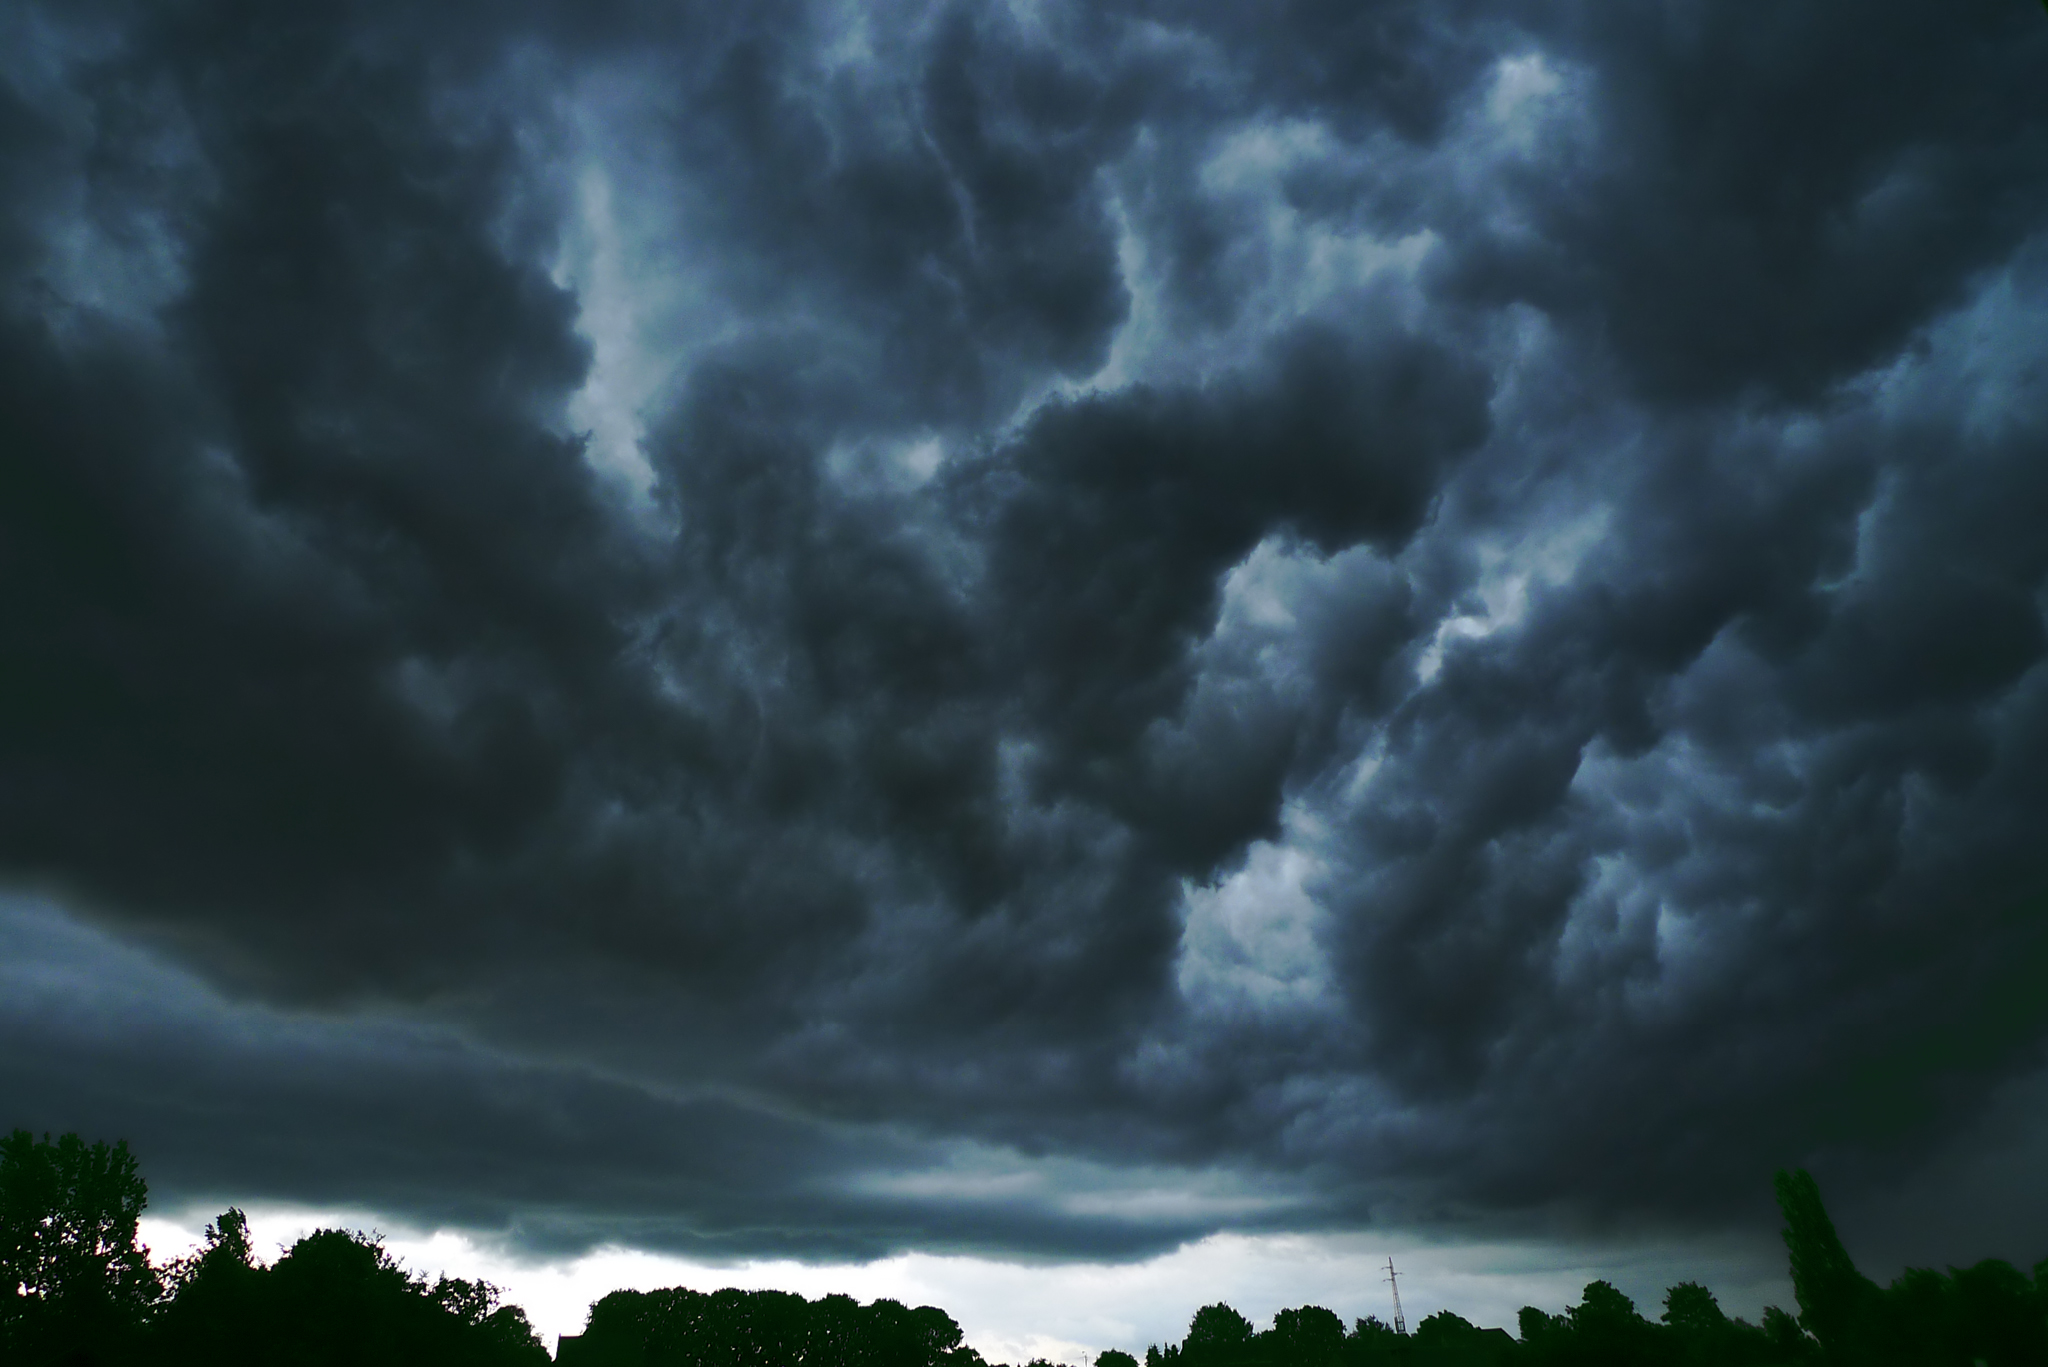
\includegraphics[width=\framewidth]{pics/thunderstorm.jpg}
% Copyright dimitri_c, http://www.freeimages.com/photo/1200003
% \paperwidth ??
\end{frame}

%%%%%%
\note{
\begin{description}
\item[N] Hallo
\item[J] Hi, na wie geht's?
\item[N] Uh, nicht so prima. Wir haben grad ziemlich viel Stress auf der Arbeit. Unsere neue Applikation wird kräftig entwickelt, aber irgendwie wird alles immer mühsamer... Guck mal hier:
\end{description}
}

%%%%%%%%%%%%%%%%%%%%%%%%%%%%%%%%%%%%%%%%%%%%%%%%%%
\begin{frame}{Unsere aktuelle Architektur}
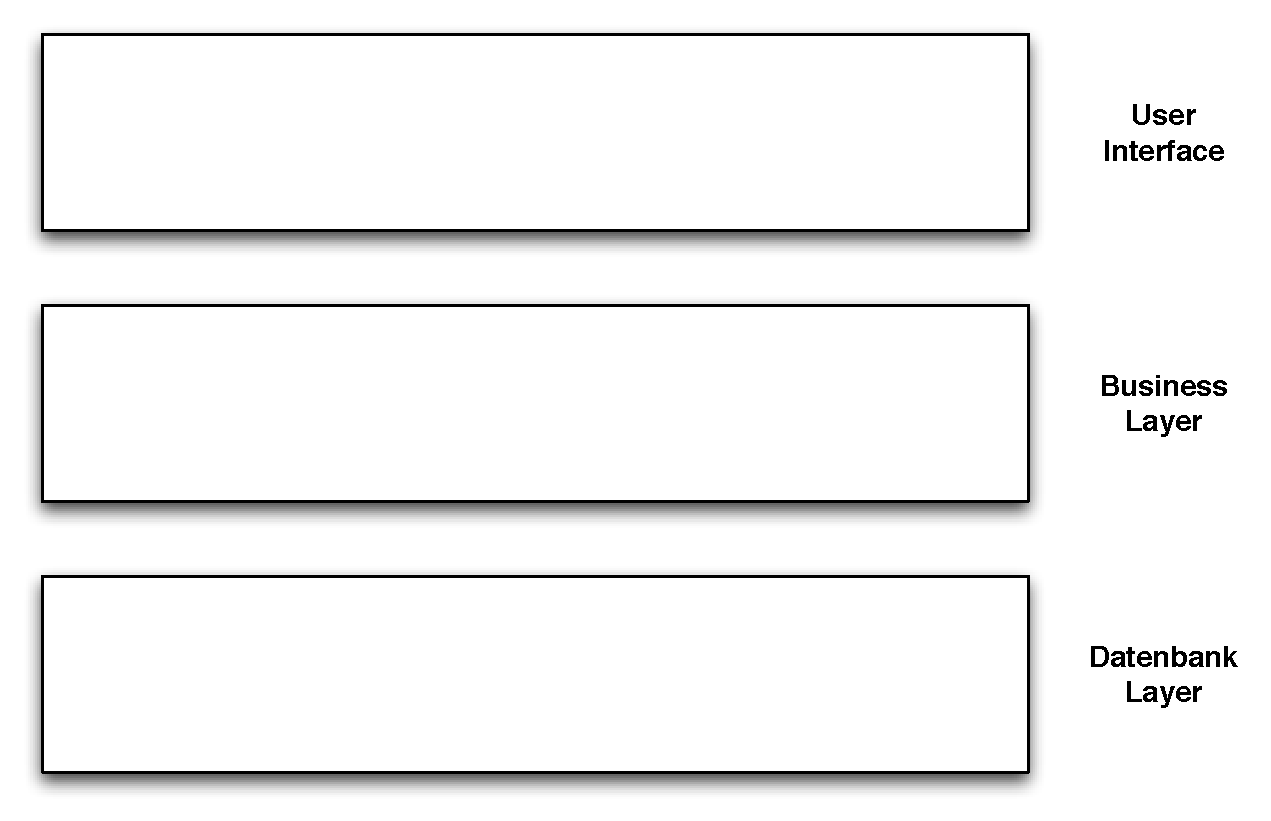
\includegraphics[width=\framewidth]{pics/Layer.pdf}

\end{frame}

%%%%%%
\note{
\begin{description}
\item[N] So sieht's gerade bei uns aus. Ganz normal, oder? UI-Layer, Business-Layer und Datenbank-Layer.
Aber irgendwie stellt sich heraus, dass unsere gesamte Logik total über die Schichten verschmiert ist. Guck mal hier:
\end{description}
}


%%%%%%%%%%%%%%%%%%%%%%%%%%%%%%%%%%%%%%%%%%%%%%%%%%
\begin{frame}{Unsere aktuelle Architektur}
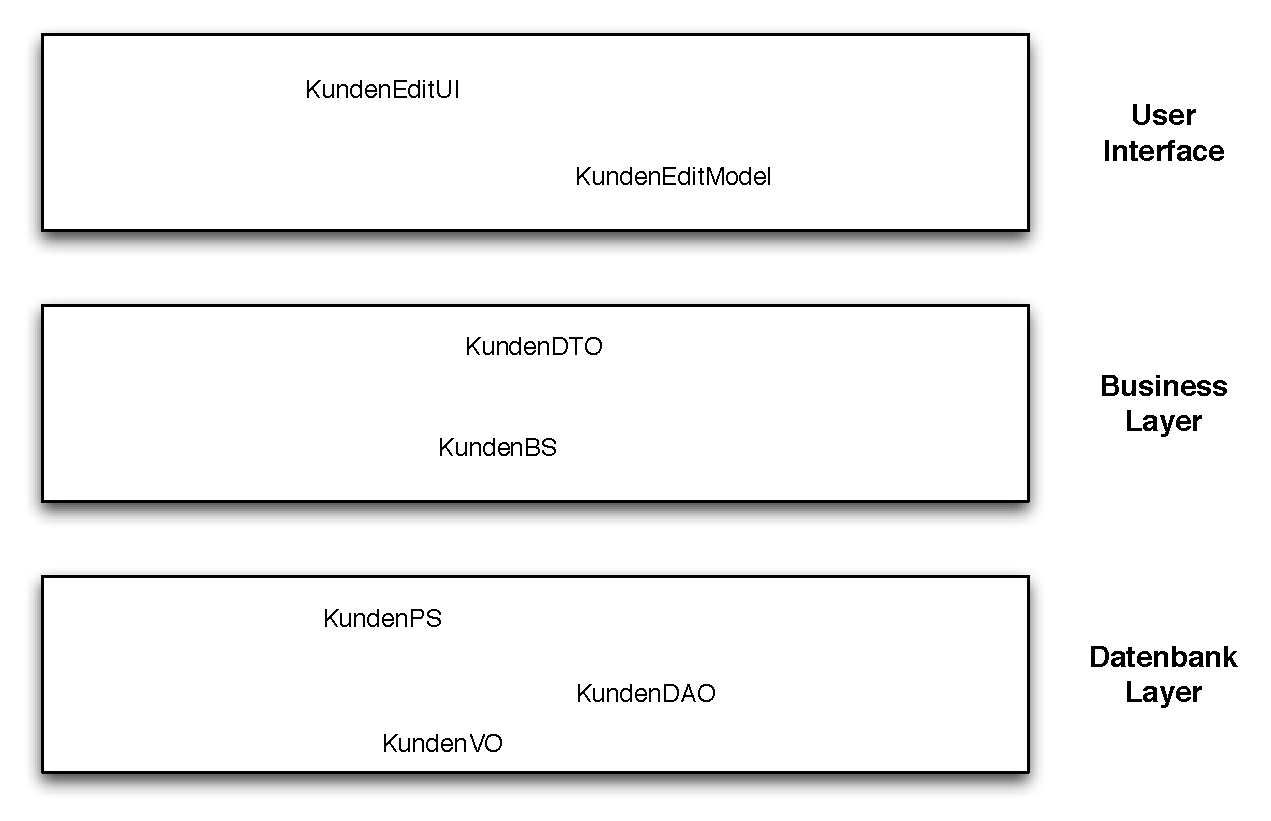
\includegraphics[width=\framewidth]{pics/LayerMitObjekten.pdf}
\end{frame}

%%%%%%
\note{
\begin{description}
\item[N] Schwierig, Tests zu schreiben / Technik auch / Auftraggeber versteht nur Bahnhof / wirft alle Abkürzungen durcheinander / alles ist aufgesplittert / Missverständnisse selbst bei Entwicklern / Jede Menge Impls und Managers
\item[J] Ja, das kenn ich gut. Wir waren auch mal in so einer Abkürzungs-Hölle.
\item[N] Waren? Das heißt, Ihr seid da rausgekommen? Und es gibt noch Hoffnung?
\item[J] Naja, geschenkt bekommen haben wir das natürlich auch nicht. Das war schon ganz schön Arbeit.
\item[N] Egal! Wie habt Ihr das gemacht, sag schon!
\end{description}
}
\note{
\begin{description}
\item[J] Naja, ... wir machen jetzt Domain-Driven Design.
\item[N] Hm, ich glaub davon hab ich schon gehört... DDD ... noch ne Abkürzung - nee, das hilft doch nicht weiter.
\item[J] Na, wart's mal ab, ich erzähl Dir einfach mal ein bisschen davon, ok?
\item[N] Na also gut... schlimmer kann's ja nicht mehr werden.
\end{description}
}

%%%%%%%%%%%%%%%%%%%%%%%%%%%%%%%%%%%%%%%%%%%%%%%%%%
\begin{frame}{Domain-Driven Design}
\begin{itemize}
\item versucht die Brücke zu schlagen zwischen Domänen-Experten und Entwicklern
\item fokussiert die Entwicklung auf die Fachlichkeit
\item gibt Entwicklern Bausteine und Werkzeuge in die Hand, um gute Anwendungen zu schreiben
\end{itemize}

% Kürzen?
%\begin{itemize}
%\item Domänen-Experten und Entwickler gemeinsam
%\item Fokus der Entwicklung auf die Fachlichkeit
%\item Bausteine und Werkzeuge für gute Anwendungen
%\end{itemize}

\end{frame}

%%%%%%
\note{
\begin{description}
\item[J] stellt die Punkte vor
\item[N] Das klingt ja sehr interessant! Aber ist das jetzt nicht wieder so ein neuer Hype?
\item[J] Nein - Teile schon Jahrzehnte alt
\item[J] DAS Buch ist über 10 Jahre alt
\item[N] OK. Aber bist Du wirklich sicher, dass das auch für uns passt?
\item[J] DDD ist besonders geeignet, wenn Fachlichkeit Kern der Anwendung / Abgegrenzte Domäne
\item[N] Das ist bei uns der Fall. Dann erzähl doch einfach mal weiter!
\end{description}
}

%%%%%%%%%%%%%%%%%%%%%%%%%%%%%%%%%%%%%%%%%%%%%%%%%%
\begin{frame}{Baustein: Entität}
\begin{itemize}
\item hat eine Identität (beschreibt das \glqq{}wer\grqq{})
\item hat einen Lebenszyklus
\item Modellierung fokussiert darauf
\item eindeutigen Identifikator festlegen
\end{itemize}
\end{frame}

%%%%%%
\note{
\begin{description}
\item[J] Identität gilt oft auch außerhalb der gerade betrachteten Software
\item[N] Ja, das kenne ich, wir modellieren Kunden, die haben natürlich auch im echten Leben einen Namen und ein Geburtsdatum
\item[J] Innerhalb des Lebenszyklus können sich Werte der Entität ändern
\item[N] Ja, das macht immer am meisten Stress, wenn die Kunden umziehen oder heiraten. Nicht so einfach, damit umzugehen...
\item[J] Genau, deswegen ist es wichtig, einen eindeutigen Identifikator festzulegen. Es könnten ja auch mal zwei Kunden denselben Namen haben.
\end{description}
}

\note{
\begin{description}
\item[N] Du meinst zum Beispiel die Objektidentität?
\item[J] Nein, da sollte man schon selbst etwas implementieren, Objektidentität passt meistens nicht genau. Insbesondere wenn man mit einer Datenbank arbeitet und immer wieder neue Instanzen einer Entität bekommt.
\item[N] Aber grundsätzlich ist es schon so, dass meine derzeitigen Datenbankobjekte alles Entitäten sind, oder? Dann verstehe ich noch nicht, was jetzt das Großartige und Neue sein soll...
\item[J] Nur Geduld! Ich vermute nämlich, dass nicht alle Deiner derzeitigen Datenbankobjekte Entitäten sind. Es gibt ja auch noch Value Objects.
\end{description}
}

%%%%%%%%%%%%%%%%%%%%%%%%%%%%%%%%%%%%%%%%%%%%%%%%%%
\begin{frame}{Baustein: Value Object}
\begin{itemize}
\item Wert
\item hat keine Identität (beschreibt \glqq{}was\grqq{}, nicht \glqq{}wer\grqq{})
\item Fachlicher Wrapper um technische Datentypen
\item bildet eine konzeptionelle Einheit
\item kann oft als Immutable implementiert werden
\begin{itemize}
\item dann ist Sharing möglich
\end{itemize}
\end{itemize}
\end{frame}

%%%%%%
\note{
\begin{description}
\item[J] Value Objects wendet man da an, wo man Werte repräsentieren will. Und wo die Identität keine Rolle spielt, also wo ich ein Value Objekt durch ein anderes identisches ersetzen kann.
\item[N] Also Du meinst Strings und ints und sowas?
\item[J] Im Prinzip schon. Aber die haben keine fachliche Semantik: Was bedeutet dieser Double, welche Werte sind hier gültig?
\item[N] Oh ja, das kenne ich. Wir haben eine Methode mit 10 Parametern, alles Doubles. Der häufigste Bug an der Stelle ist, dass irgendjemand mal wieder die Werte in der falschen Reihenfolge übergeben hat...
\end{description}
}
\note{
\begin{description}
\item[J] Und deswegen ist es sinnvoll, fachliche Wrapper-Klassen zu erstellen, die die Semantik ausdrücken. Simple Beispiele sind Geldbetrag oder Prozentsatz.
Interessant dabei ist, dass man Value Objects oft als immutable implementieren kann, d.~h.~dass man das Objekt nach der Erzeugung nicht mehr verändern kann.
\item[N] Hm, aber was ist, wenn sich jetzt was ändert, zum Beispiel die Gesamtsumme in meinem Warenkorb?
\end{description}
}

\note{
\begin{description}
\item[J] Da kann ich einfach einen neuen Geldbetrag mit der neuen Gesamtsumme bauen und den alten dadurch ersetzen. Und die Implementierung meines Value Objects wird dadurch viel einfacher. Man kann sogar häufig vorkommende Value Objects wiederverwenden - das ist ungefährlich, denn sie können ja nicht verändert werden.
\item[N] Ah, klingt interessant! Wir haben ganz oft einen Preis von 99 Cent, da könnte ich dann immer dasselbe Value Object verwenden, oder?
\item[J] Ja, zum Beispiel.

\item[N] Mensch, danke für die vielen Infos! Jetzt bin ich mal gespannt, wie wir das Ganze bei uns im Team umsetzen können. Tschüs, ich muss los!
\end{description}
Gehen ab.
}

%%%%%%%%%%%%%%%%%%%%%%%%%%%%%%%%%%%%%%%%%%%%%%%%%%
\begin{frame}{Einige Wochen später...}

\includegraphics[width=\framewidth]{pics/dandelions.jpg}
% Copyright Krappweis, http://www.freeimages.com/photo/1429166
\end{frame}

%%%%%%
\note{
\begin{description}
\item[J] Hallo, schön Dich wiederzusehen! Wie läuft's denn so mit Domain-Driven Design?
\item[N] Oh, sehr gut! Wir haben inzwischen einige unserer Probleme in den Griff bekommen und auch coole neue Sachen entdeckt.
\item[J] Das ist ja schön zu hören! Magst Du mir was davon erzählen?
\end{description}
}

%%%%%%%%%%%%%%%%%%%%%%%%%%%%%%%%%%%%%%%%%%%%%%%%%%
\begin{frame}{Neues über Value Objects}
\begin{itemize}
\item aus Entitäten auslagern
\item können auch komplexer aufgebaut sein
\item entwickeln sich zu \glqq{}Code-Magneten\grqq{}
\end{itemize}
\end{frame}

%%%%%%
\note{
\begin{description}
\item[N] wir hatten ziemlich viele riesige Entitäten, z. B. hat unser Kunde alle Angaben über ihn direkt als Attribute gehabt: Alle Namens- und Adressbestandteile, Telefonnummer, Kreditkartennummer und was noch alles. Davon haben wir den Großteil herausgezogen und in spezialisierten Value Objects untergebracht. Der Kunde kennt jetzt nur noch diese Value Objects und nicht mehr die Details.
\item[N] Ein interessanter Nebeneffekt: Wir machen jetzt auch komplexe Value Objects, nicht nur simple Wrapper. Wie zum Beispiel unsere Adresse.
\end{description}
}

\note{
\begin{description}
\item[J] Eine Adresse ist ein gutes Beispiel für ein komplexes Value Object in der Domäne \glqq{}Online-Store\grqq{}. Denk nur dran, dass es in anderen Domänen ganz anders sein kann. In einer Grundstücksverwaltung oder in einer Briefzustellungssoftware wird man Adressen vermutlich eher als Entitäten modellieren. 
\item[N] Hm...
\item[J] Aber ich hab Dich unterbrochen. Was hast Du denn sonst noch so rausgefunden?
\end{description}
}

\note{
\begin{description}
\item[N] Das coolste ist: Die Value Objects ziehen den Code förmlich an! Alles, was mit einem Value Object zu tun hat, implementieren wir dort als Methode: z. B. Validierung oder das Herausziehen von Teilaspekten (... ?!)
Früher war dieser Code im ganzen System verstreut, und meistens hat man ihn nicht wiedergefunden, wenn man ihn gebraucht hat, und hat alles nochmal implementiert, und nochmal... Jetzt gibt es einen klaren Platz für diesen Code, das ist super!
\item[J] Mir scheint, Ihr seid auf einem richtig guten Weg!
\item[N] Aber es knirscht auch noch ganz schön an vielen Stellen.
\end{description}
}

\note{
\begin{description}
\item[J] Wo denn zum Beispiel?
\item[N] Naja, wir Entwickler kommen noch nicht so gut klar mit den Leuten vom Fachbereich. Sie sprechen eine ganz andere Sprache als wir, zum Beispiel sagen sie "Artikel", und das heißt bei uns im Code "Bestellposition". Einer von uns hat das gut im Griff und spielt immer den Übersetzer. Aber wenn der nicht da ist, läuft echt gar nix.
\item[J] Dass eine gemeinsame Sprache sehr wichtig ist, das ist auch ein Schwerpunkt von DDD.
\end{description}
}



%%%%%%%%%%%%%%%%%%%%%%%%%%%%%%%%%%%%%%%%%%%%%%%%%%
\begin{frame}{Die allgegenwärtige Sprache}
\begin{itemize}
\item Fachbegriffe überall verwenden, auch im Code!
\item Glossar
\end{itemize}
\end{frame}

%%%%%%
\note{
\begin{description}
\item[J] Du hast ja selbst schon festgestellt, wie wichtig und schwierig die Sprache ist.
\item[N] x
\item[J] x
\end{description}
}

% Hier geht's weiter...

% FAZIT:
%%%%%%%%%%%%%%%%%%%%%%%%%%%%%%%%%%%%%%%%%%%%%%%%%%
\begin{frame}{Achtung!}
\begin{itemize}
\item Technisches nicht hinten runterfallen lassen
\end{itemize}
\end{frame}

%%%%%%
\note{
\begin{description}
\item[N] x
\item[J] x
\end{description}
}


%%%%%%%%%%%%%%%%%%%%%%%%%%%%%%%%%%%%%%%%%%%%%%%%%%
\begin{frame}{Was man beherzigen darf}
\begin{itemize}
\item x
\end{itemize}
\end{frame}

%%%%%%
\note{
\begin{description}
\item[N] x
\item[J] x
\end{description}
}



% TEMPLATE:
%%%%%%%%%%%%%%%%%%%%%%%%%%%%%%%%%%%%%%%%%%%%%%%%%%
\begin{frame}{x}
\begin{itemize}
\item x
\end{itemize}
\end{frame}

%%%%%%
\note{
\begin{description}
\item[N] x
\item[J] x
\end{description}
}


%%%%%%%%%%%%%%%%%%%%%%%%%%%%%%%%%%%%%%%%%%%%%%%%%%
{
\usebackgroundtemplate{
\includegraphics[width=\paperwidth,height=\paperheight]{background-slide.png}}
\begin{frame}{Vielen Dank!}

        Folien auf GitHub:
        \vspace{-0.8em}
        \begin{center}
                \url{https://github.com/NicoleRauch/DomainDrivenDesign}
        \end{center}

        \begin{block}{Jens Borrmann}
        \begin{description}[Twitterxx]
                \item[E-Mail]  \href{mailto:jens.borrmann@msg-gillardon.de}{\texttt{jens.borrmann@msg-gillardon.de}}
                \item[Twitter] \href{http://twitter.com/jborrmann}{\texttt{@jborrmann}}
        \end{description}
        \end{block}
        \begin{block}{Nicole Rauch}
        \begin{description}[Twitterxx]
                \item[E-Mail]  \href{mailto:nicole.rauch@msg-gillardon.de}{\texttt{nicole.rauch@msg-gillardon.de}}
                \item[Twitter] \href{http://twitter.com/NicoleRauch}{\texttt{@NicoleRauch}}
        \end{description}
        \end{block}
\end{frame}
}
